\documentclass[a4paper,10pt]{article}
\usepackage[english]{babel}
\usepackage[utf8]{inputenc}
\usepackage{url}
\usepackage[margin=1in]{geometry}
\usepackage{enumitem}

\usepackage[nottoc]{tocbibind}
\usepackage{fancyvrb} 
\usepackage{float}
\usepackage{graphicx}
\usepackage{subcaption}
\usepackage{color}
\usepackage{booktabs}
\usepackage{listings}

\title{Combinatorial Optimization\\Homework 3 – Experimental Measurements}
\author{Matyáš Skalický\\skalimat@fit.cvut.cz}

\begin{document}
\maketitle
\tableofcontents
\medskip


\section{Measured Algorithms}

Baseline exact method is the \textbf{brute-force} algorithm that simply iterates all possible solutions without any speedups.

The \textbf{branch\&bound} extends the brute-force with 2 speedups. We stop when the current candidate already exceeds the capacity of a bag. Also, we don't recurse further when the cost sum of the items that can be added into the bag is lower than the best found solution.

The dynamic programming approach is based on the \textbf{decomposition by cost}. This solution is based on memoization by the recursive function calls by returning the maximum value from the tested branches on return.

The \textbf{greedy} heuristic simply adds the items with the highest cost/weight ratio until the capacity of the bag is reached. This is the only algorithm that doesn't always result in the optimal solution.

\section{Measured Variables}
For the pilot experiments, I've chosen to benchmark all algorithms on the instances of size $24$. The generator's maximum weight $W$ is set to $3000$ as well as maximum price $C$.

In the following experiments, we will try to measure how time and the solution quality depend on the generator inputs. Also, we will look how robust each algorithm is against permutations in the algorithm inputs.

\begin{itemize}
	\item Ratio of bag capacity to summary weight. (\lstinline{cw_ratio} $\in [0, 2]$)
	\item Correlation between price and weight. (\lstinline{pw_corr} $\in [0, 1]$)
	\item Granularity and distribution of weights. (\lstinline{w_dist} $\in [0, 2]$)
\end{itemize}

We will try to put emphasis on the hypothesis below:

\section{Experiments}
We will measure the effect of each variable separately. We will generate 10 problem instances for each algorithm with each weight.

\subsection{Robustness}
First, we will try to answer the robustness (invariance to order of input items) of each algorithm. We will use default generator values mentioned above. We will generate 500 instances and calculate 10 permutations for each algorithm.

\subsection{Pilot Experiments}

 We will not measure the permutations in the pilot experiments.

%\begin{figure}[!htb]
%	\centering
%  	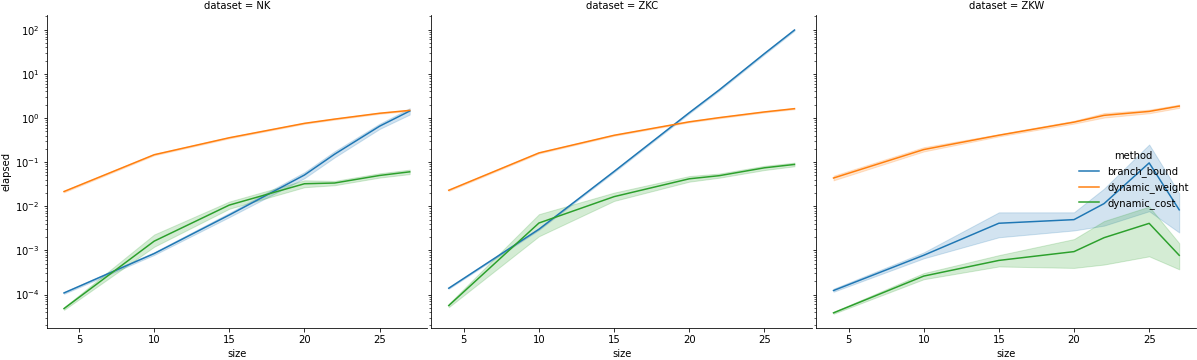
\includegraphics[width=\textwidth]{images/exacts_comparison.png}
%	\caption{Comparison of the exact algorithms: branch\&bound, decomposition by cost and weight}
%	\label{exacts_comparison}
%\end{figure}

\subsection{Detailed Experiments}


\section{Discussion and Takeoffs}


\end{document}